\section{Materials and Methods}

\subsection{Benchmark Corpora and Industrial Data Provenance}
To rigorously assess automated classification performance across diverse operational envelopes, this investigation employs three heterogeneous requirements corpora comprising a cumulative volume of 8,654 authentic software specifications: the canonical PROMISE repository, the extended PROMISE-EXP dataset, and the large-scale industrial FNFC corpus. The PROMISE benchmark represents the classical gold standard in empirical requirements engineering research, consisting of 625 natural language requirement statements gathered across multiple real-world software projects. Within PROMISE, specifications are annotated into functional requirements and ten distinct non-functional quality categories, including performance, security, usability, maintainability, and operational constraints. The PROMISE-EXP corpus expands upon the canonical dataset, compiling 969 software specifications distributed across twelve authentic software engineering requirement categories, capturing multi-tiered constraint dependencies and diverse technical domains. To evaluate architectural scalability under authentic enterprise conditions, the industrial FNFC benchmark encompasses 7,060 requirements extracted from commercial software systems, representing an extensive operational scale rarely evaluated in bio-inspired literature.

A pervasive characteristic of software requirements corpora is the presence of acute class distribution skew. In industrial engineering practice, functional specifications dominate technical documentation, whereas safety-critical quality attributes appear as sparse, high-consequence requirements. To quantify the extent of distributional disparity across the three corpora, the class imbalance severity ratio is formally defined as:
\begin{equation}
IR = \frac{\max_{c \in \mathcal{C}} N_c}{\min_{c \in \mathcal{C}} N_c}
\end{equation}
where $\mathcal{C}$ denotes the complete set of target classes and $N_c$ represents the total sample frequency of class $c$. Across the evaluated datasets, $IR$ ranges from moderate disparity in binary industrial partitions to extreme skews exceeding 70:1 in fine-grained quality subcategories.

\begin{table}[htbp]
\centering
\caption{Comprehensive descriptive statistics and class distribution profiles across the benchmark corpora.}
\label{tab:dataset_statistics}
\small
\resizebox{\textwidth}{!}{%
\begin{tabular}{lcccccc}
\toprule
Corpus Identifier & Sample Volume ($N$) & Target Classes & Majority Class (Count, \%) & Minority Class (Count, \%) & Imbalance Ratio ($IR$) & Lexical Vocabulary \\
\midrule
PROMISE Canonical & 625 & 12 & Functional (255, 40.80\%) & Fault Tolerance (10, 1.60\%) & 25.50:1 & 1,420 tokens \\
PROMISE-EXP Extended & 969 & 12 & Functional (444, 45.82\%) & Portability (12, 1.24\%) & 37.00:1 & 2,150 tokens \\
FNFC Industrial & 7,060 & 2 & Functional (6,030, 85.41\%) & Non-Functional (1,030, 14.59\%) & 5.85:1 & 8,920 tokens \\
\bottomrule
\end{tabular}%
}
\end{table}

\begin{figure}[htbp]
\centering
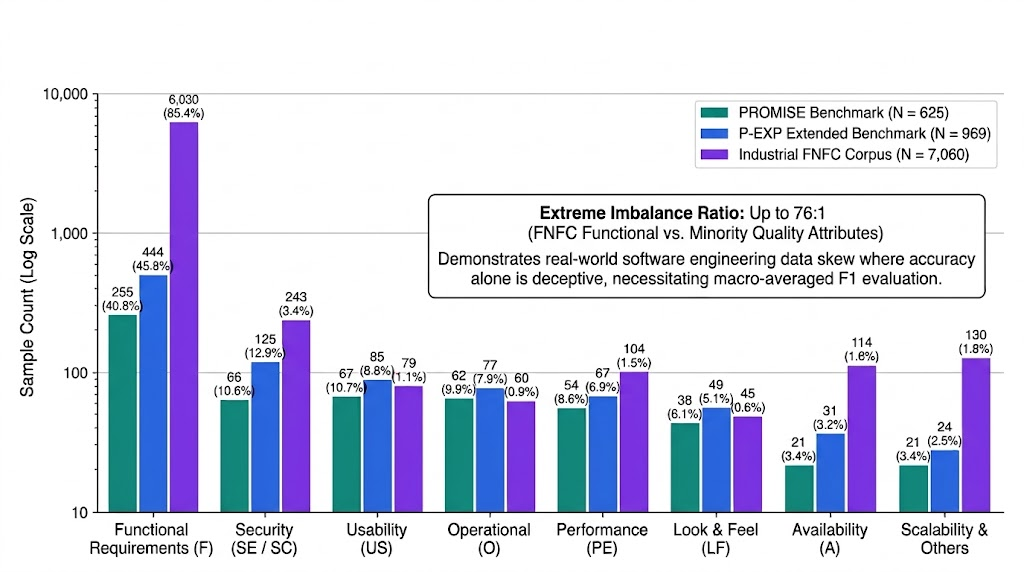
\includegraphics[width=\textwidth]{figures/fig3_dataset_imbalance.png}
\caption{Comprehensive class frequency distribution and severity imbalance profiles across the tri-dataset benchmark corpora: (a) Canonical PROMISE ($N=625$), (b) Extended PROMISE-EXP ($N=969$), and (c) Industrial FNFC ($N=7,060$), demonstrating real-world distribution skew motivating macro-averaged evaluation.}
\label{fig:dataset_imbalance}
\end{figure}

\subsection{Dynamic Syntactic-Semantic Dinucleotide Codon Grammar}
Prior bio-inspired classification attempts mapped requirement tokens into isolated single nucleotides, treating each character as an independent categorical label and thereby forfeiting critical syntactic dependencies. To resolve this representational limitation, DNA+ formulates a dynamic syntactic-semantic dinucleotide codon grammar. In natural language software engineering, requirement statements are inherently governed by coupled grammatical structures: a primary operational anchor that denotes the imperative action or requirement modality, and an auxiliary constraint dependency that delineates the quality attribute, operational condition, or security boundary.

The framework defines an alphabet of four nucleotide bases $\Sigma = \{A, T, C, G\}$, where each base corresponds to a distinct functional or quality dimension based on comprehensive semantic lexicons. Nucleotide $A$ encapsulates functional actions and imperative obligations; nucleotide $T$ represents human-computer interaction, usability, and visual aesthetics; nucleotide $C$ denotes cybersecurity, confidentiality, integrity, and regulatory compliance; and nucleotide $G$ captures performance, temporal deadlines, throughput, scalability, and system reliability. For each requirement statement $r$, the dynamic mapper detects the primary modal verb and computes lexical density scores across the four base vocabularies. The statement is formally projected into a dinucleotide codon space through the projection operator $\Psi$:
\begin{equation}
\Psi(r) = \langle b_1(w_{\text{anchor}}), b_2(w_{\text{aux}}) \rangle \in \Sigma^2
\end{equation}
where $b_1$ and $b_2$ represent the primary and auxiliary nucleotide bases derived from sorted contextual evidence scores. When a statement exhibits overwhelming evidence for a single semantic dimension without secondary constraints, the operator yields a homozygous dinucleotide codon ($b_1 = b_2 \in \{AA, TT, CC, GG\}$). Conversely, compound specifications containing intersecting quality demands produce heterozygous dinucleotide pairs, alphabetically standardized to preserve canonical symmetry ($b_1 b_2 \in \{AC, AG, AT, CG, CT, GT\}$).

\begin{table}[htbp]
\centering
\caption{Dynamic syntactic-semantic dinucleotide codon codebook and linguistic mapping specifications.}
\label{tab:codon_codebook}
\small
\resizebox{\textwidth}{!}{%
\begin{tabular}{lccp{5.5cm}p{6.5cm}}
\toprule
Codon Permutation & Primary Base ($b_1$) & Auxiliary Base ($b_2$) & Syntactic-Semantic Constraint Role & Exemplar Requirement Triggers \\
\midrule
AA & Functional ($A$) & Functional ($A$) & Pure Imperative / Operational Capability & shall provide, must calculate, execute, process \\
AT & Functional ($A$) & Usability ($T$) & User-Centric Functional Interaction & user shall navigate, system displays screen icon \\
AC & Functional ($A$) & Security ($C$) & Policy-Constrained Functional Execution & system must verify password, authenticate session \\
AG & Functional ($A$) & Performance ($G$) & Time-Constrained Operational Throughput & shall respond within 2 seconds, process in 500 ms \\
TT & Usability ($T$) & Usability ($T$) & Pure Ergonomics / Visual Aesthetic & accessible theme, simple intuitive interface layout \\
TC / CT & Usability ($T$) & Security ($C$) & Secure Human-Interface Interaction & login dialog, encrypted session form, credential prompt \\
TG / GT & Usability ($T$) & Performance ($G$) & Interface Rendering Latency & dashboard refresh rate, screen render speed \\
CC & Security ($C$) & Security ($C$) & Cryptographic / Regulatory Enforcement & 256-bit AES encryption, HIPAA compliance audit \\
CG & Security ($C$) & Performance ($G$) & High-Throughput Secure Processing & secure transactions per second, TLS overhead \\
GG & Performance ($G$) & Performance ($G$) & Scalability / Availability Envelopes & 99.9\% uptime, 10,000 concurrent user threads \\
\bottomrule
\end{tabular}%
}
\end{table}

\subsection{Synthetic Biological Sequence Generation and FASTA Structuring}
Following dinucleotide target identification, the framework synthesizes authentic macromolecular biological nucleotide sequences directly from the normalized natural language requirement text. Preprocessing initiates with contraction expansion, lowercasing, and alphanumeric tokenization, stripping punctuation while preserving numerical parameters that signify quantitative performance thresholds. Each extracted token $w_i$ is mapped against the inverted base dictionary. Tokens matching domain actions resolve to base $A$, usability and interface keywords map to base $T$, security and compliance terms resolve to base $C$, and temporal units, latency values, and scalability metrics map to base $G$. Tokens that do not match the domain lexicon are bypassed, while quantitative numbers directly append nucleotide $G$ to reflect technical metric constraints.

The synthesized nucleotide string $S(r)$ is constructed via sequential string concatenation across all mapped tokens:
\begin{equation}
S(r) = \bigoplus_{i=1}^{M} \text{Base}(w_i) = c_1 c_2 \dots c_M, \quad c_i \in \{A, T, C, G\}
\end{equation}
where $M$ denotes the total number of mapped tokens in requirement $r$. If a terse requirement produces no vocabulary matches, a minimal functional motif $A$ is assigned to prevent null sequence exceptions. The resulting synthetic chains are structured into standard biological FASTA records, complete with unique sequence identification headers and provenance metadata, establishing a persistent knowledge base suitable for downstream bioinformatics toolchains.

\begin{figure}[htbp]
\centering
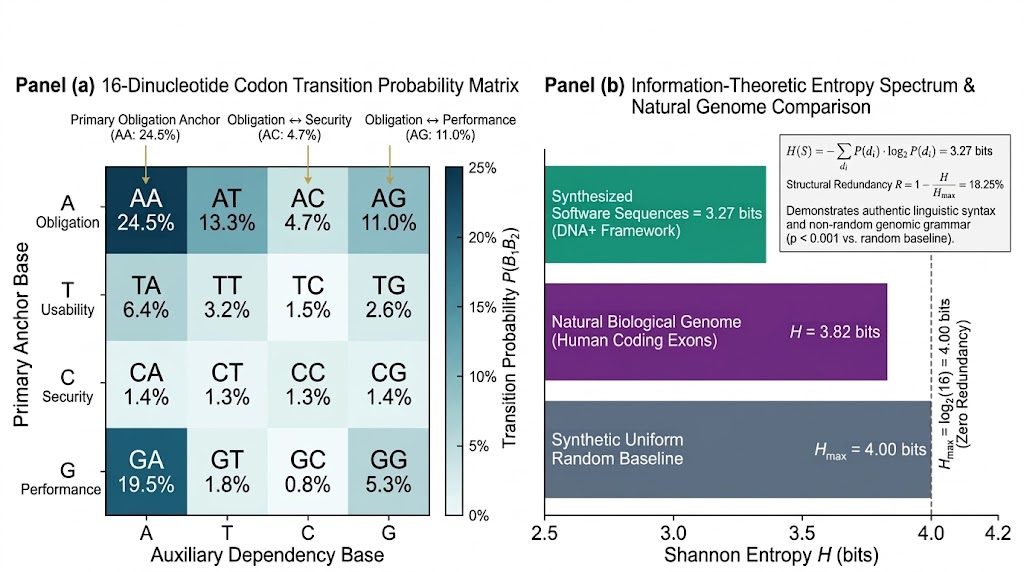
\includegraphics[width=\textwidth]{figures/fig2_codon_landscape.png}
\caption{Empirical biological dinucleotide landscape: (a) 16-state dinucleotide transition probability matrix extracted from synthetic software sequences, and (b) Information-theoretic Shannon sequence entropy spectrum ($H=3.27$ bits, $R=18.25\%$) confirming non-random genomic grammar matching biological sequence constraints.}
\label{fig:codon_landscape}
\end{figure}

\subsection{Alignment-Free Genomic Physicochemical Feature Extraction}
To transform synthetic biological sequences into discriminative numeric feature vectors without incurring the computational bottlenecks of pairwise sequence alignment, DNA+ deploys alignment-free oligonucleotide statistics and information-theoretic metrics. The feature extractor analyzes biological sequences across three complementary analytical tiers: single-nucleotide monomer frequencies, dinucleotide dimer transition odds, and global physicochemical sequence properties.

At the monomer tier ($k=1$), the relative frequency of each nucleotide base $b \in \{A, T, C, G\}$ is computed over sequence length $|S(r)|$:
\begin{equation}
f(b) = \frac{N(b)}{|S(r)|}, \quad \forall b \in \{A, T, C, G\}
\end{equation}
where $N(b)$ represents the absolute occurrence count of base $b$. At the dimer tier ($k=2$), the extractor enumerates all sixteen contiguous dinucleotide permutations $XY \in \{AA, AT, \dots, GG\}$, capturing local sequential transition dynamics:
\begin{equation}
f(XY) = \frac{N(XY)}{\max(1, |S(r)| - 1)}, \quad \forall X, Y \in \{A, T, C, G\}
\end{equation}
To quantify nucleotide balance, the framework computes the biological GC-content percentage, representing the proportion of guanine and cytosine bases within the sequence:
\begin{equation}
\text{GC}(S) = \frac{N(G) + N(C)}{|S(r)|} \times 100\%
\end{equation}
In biological genomics, GC-content governs thermal stability and sequence complexity. Within software requirement sequences, elevated GC-content directly signals dense concentrations of technical performance constraints and security protocols. The framework further computes the AT/GC skew ratio and logarithmic sequence length scaling:
\begin{equation}
\theta_{\text{ratio}}(S) = \frac{N(A) + N(T)}{N(G) + N(C) + \epsilon}, \quad L(S) = \ln(|S(r)| + 1)
\end{equation}
where $\epsilon = 10^{-5}$ prevents division by zero in GC-devoid sequences. 

To evaluate syntactic diversity and vocabulary unpredictability within the synthesized sequences, the framework incorporates Shannon information entropy [11]:
\begin{equation}
H(S) = -\sum_{b \in \{A, T, C, G\}} f(b) \log_2 f(b)
\end{equation}
The informational redundancy $R(S) = 1 - (H(S) / \log_2 4)$ quantifies deviations from uniform nucleotide distribution. This formulation draws upon foundational genomic signature theory [12], which proved that dinucleotide frequency distributions constitute invariant species-specific signatures, as well as computational linguistics demonstrating that non-coding DNA sequences follow formal statistical language structures [13]. Furthermore, alignment-free sequence statistics provide invariant distance metrics without alignment overhead [14], while $k$-mer counting captures local sequence regulatory motifs with high computational scalability [15]. In total, the genomic extraction module generates a compact 23-dimensional physicochemical profile ($4\text{ monomers} + 16\text{ dimers} + \text{GC-content} + \text{AT/GC ratio} + \text{log-length}$).

\subsection{Multimodal Feature Manifold Fusion and Dimensionality Synthesis}
While genomic sequence attributes provide structural and syntactic regularity, they do not directly model high-level semantic context or nuanced domain vocabularies. To achieve comprehensive representation, DNA+ synthesizes a multimodal feature manifold by integrating the 23-dimensional genomic vector with classical lexical frequencies and dense contextual transformer embeddings.

\begin{figure}[htbp]
\centering
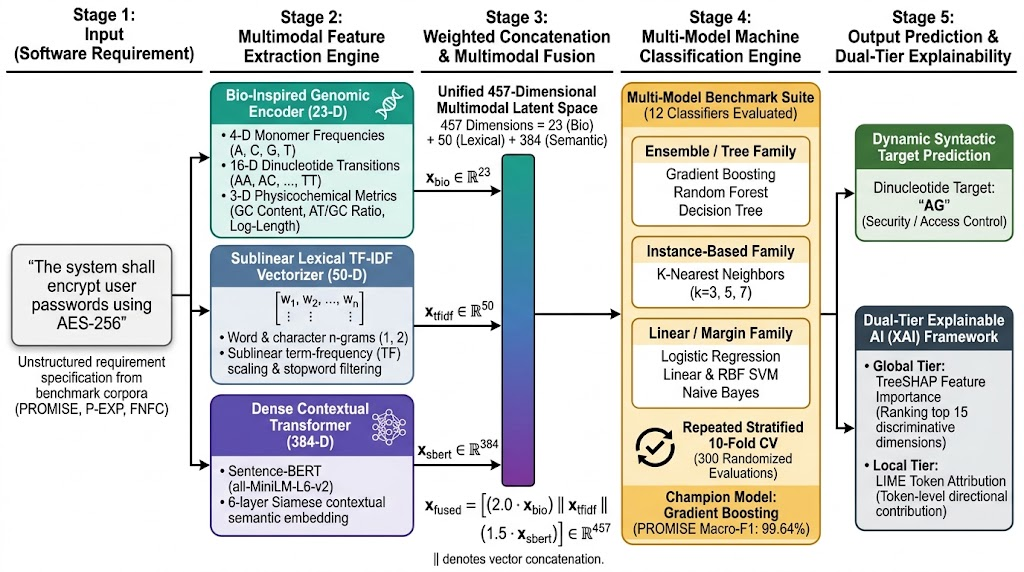
\includegraphics[width=\textwidth]{figures/fig1_system_architecture.png}
\caption{End-to-end multimodal pipeline architecture of the proposed DNA+ framework: Stage 1 Requirements Ingestion; Stage 2 Feature Extraction (23-D Genomic, 50-D TF-IDF, 384-D SBERT); Stage 3 Weighted Manifold Synthesis (457-D); Stage 4 Multi-Algorithm Benchmark Suite (12 Classifiers); and Stage 5 Explainable Prediction via Dual-Tier TreeSHAP and LIME.}
\label{fig:system_architecture}
\end{figure}

The lexical branch extracts salient unigram and bigram patterns using term frequency-inverse document frequency vectorization. To suppress the disproportionate influence of frequently repeated administrative terms while amplifying discriminative technical terms, sublinear scaling is applied:
\begin{equation}
\text{TF-IDF}(t, d) = \left(1 + \ln(\text{tf}(t, d))\right) \cdot \ln\left(\frac{1 + N_D}{1 + \text{df}(t)}\right) + 1
\end{equation}
where $\text{tf}(t, d)$ denotes term frequency in document $d$, $\text{df}(t)$ represents document frequency, and $N_D$ is the total corpus size. The top fifty most informative lexical features are retained, yielding a 50-dimensional lexical feature vector $\mathbf{v}_{\text{tfidf}}^{50}$.

To capture abstract semantic concepts and semantic associations across requirement statements, the contextual semantic branch employs a pre-trained Siamese transformer network, specifically the all-MiniLM-L6-v2 Sentence-BERT architecture. The model processes the cleaned requirement string through multi-head self-attention layers, generating a continuous 384-dimensional dense semantic embedding via mean pooling over token representations:
\begin{equation}
\mathbf{e}_{\text{sbert}}(r) = \text{MeanPooling}\left(\text{TransformerEncoder}(r)\right) \in \mathbb{R}^{384}
\end{equation}

The three constituent representations are synthesized into a unified 457-dimensional multimodal feature manifold $\mathbf{z}_{\text{multimodal}}$. To ensure that structural genomic properties exert sufficient influence alongside dense semantic embeddings, an empirical weighting coefficient is applied:
\begin{equation}
\mathbf{z}_{\text{multimodal}} = \left[ 2.0 \cdot \mathbf{v}_{\text{genomic}}^{23} \;\|\; 1.0 \cdot \mathbf{v}_{\text{tfidf}}^{50} \;\|\; 1.5 \cdot \mathbf{e}_{\text{sbert}}^{384} \right] \in \mathbb{R}^{457}
\end{equation}
where $\|$ denotes horizontal vector concatenation. The $2.0\times$ amplification factor on genomic dimensions reinforces structural sequence signals, while the $1.5\times$ scaling on Sentence-BERT maintains contextual fidelity, establishing a discriminative manifold summarized in Table 3.

\begin{table}[htbp]
\centering
\caption{Multimodal feature manifold decomposition and dimensionality allocation ($457$-D).}
\label{tab:feature_manifold}
\small
\resizebox{\textwidth}{!}{%
\begin{tabular}{lccp{5.5cm}p{6.5cm}}
\toprule
Feature Module & Dimensions & Relative Weight & Mathematical Core Formulation & Extraction Rationale and Representation Scope \\
\midrule
Genomic Monomers ($k=1$) & 4 & $2.0\times$ & Nucleotide Base Counts ($A, T, C, G$) / $|S|$ & Macro-level functional vs. quality composition \\
Genomic Dimers ($k=2$) & 16 & $2.0\times$ & Dimer Transition Counts / $(|S| - 1)$ & Local transition dynamics and codon sequence motifs \\
Physicochemical Properties & 3 & $2.0\times$ & GC-Content, AT/GC Skew Ratio, $\ln(|S| + 1)$ & Sequence information density and structural stability \\
Lexical TF-IDF Vector & 50 & $1.0\times$ & Sublinear Term Frequency $\times$ Inverse Document Frequency & Salient domain-specific technical vocabulary and n-grams \\
Dense Contextual SBERT & 384 & $1.5\times$ & Mean-Pooled Siamese Transformer Hidden States & High-order abstract contextual semantics and polysemy \\
\midrule
Full Multimodal Manifold & 457 & --- & Concatenated Weighted Feature Matrix ($\mathbf{z}_{\text{multimodal}}$) & Unified bio-inspired sequence and semantic representation \\
\bottomrule
\end{tabular}%
}
\end{table}

\subsection{Multi-Algorithm Ensemble Learning Architecture}
To evaluate classification performance across distinct inductive biases, the multimodal feature manifold is ingested by a suite of twelve supervised machine learning classifiers: Random Forest, Gradient Boosting, AdaBoost, Decision Trees, Linear Support Vector Machines, Radial Basis Function Support Vector Machines, Logistic Regression, Gaussian Naive Bayes, Multinomial Naive Bayes, and $k$-Nearest Neighbors ($k \in \{3, 5, 7\}$).

Given the severe class imbalance documented in Section 2.1, conventional loss functions frequently bias predictions toward majority classes. While synthetic oversampling methods such as SMOTE generate artificial interpolation samples [16], empirical software engineering research demonstrates that synthetic data generation risks distorting real-world feature boundaries [17,18]. Consequently, DNA+ maintains raw class distributions and integrates cost-sensitive class re-weighting directly into model objectives. For each class $c \in \mathcal{C}$, an inverse frequency weight $w_c = N / (|\mathcal{C}| \cdot N_c)$ penalizes misclassifications on minority samples. The ensemble decision rule optimizes posterior class probabilities across the constituent learners:
\begin{equation}
\hat{y} = \arg\max_{c \in \mathcal{C}} \sum_{m=1}^{M} w_m P_m(y = c \mid \mathbf{z}_{\text{multimodal}})
\end{equation}
where $w_m$ denotes the normalized performance weight assigned to classifier $m$, and $P_m(y = c \mid \mathbf{z}_{\text{multimodal}})$ represents the calibrated class posterior probability.

\subsection{Dual-Tier Explainable AI Formulation: Global TreeSHAP and Local LIME}
To ensure that predictions generated over the 457-dimensional multimodal manifold remain fully transparent to software engineering practitioners, DNA+ integrates a dual-tier explainable artificial intelligence diagnostic suite combining global feature attribution with local instance-level explanations.

At the global tier, the framework utilizes TreeSHAP, an exact polynomial-time implementation of Shapley Additive Explanations for tree-based ensemble models. Grounded in cooperative game theory, TreeSHAP allocates fair marginal contribution values $\phi_i$ to each feature $i$ across all possible feature subsets $\mathcal{F}$:
\begin{equation}
\phi_i(f, \mathbf{z}) = \sum_{S \subseteq \mathcal{F} \setminus \{i\}} \frac{|S|!(|\mathcal{F}| - |S| - 1)!}{|\mathcal{F}|!} \left[ f(S \cup \{i\}) - f(S) \right]
\end{equation}
where $f(S)$ represents model expectation conditioned on subset $S$. TreeSHAP quantifies the global impact of monomer frequencies, dinucleotide transitions, GC-content, and individual SBERT dimensions across the entire corpus.

At the local tier, the framework deploys Local Interpretable Model-agnostic Explanations (LIME) to provide requirements engineers with instance-specific justifications. For a given requirement $x$, LIME constructs an interpretable linear surrogate model $g \in G$ by minimizing local fidelity loss over perturbed neighborhood samples $z \in \mathcal{Z}$:
\begin{equation}
\xi(x) = \arg\min_{g \in G} \mathcal{L}(f, g, \pi_x) + \Omega(g)
\end{equation}
where $\pi_x(z) = \exp(-D(x, z)^2 / \sigma^2)$ defines an exponential distance proximity kernel, and $\Omega(g)$ penalizes surrogate model complexity. Through this dual-tier architecture, DNA+ substantiates that classification decisions are driven by legitimate domain constraints and biological sequence grammar rather than spurious correlation artifacts.